%%%%%%%%%%%%%%%%%%%%%%%%%%%%%%%%%%%%%%%%%%%%%%%%%%%%%%%%%%%%%%%%%%%%%%%%%
%%%% Plantilla realizada por César Martínez cesar.martinez@udlap.mx %%%%%
%%%%%%%%%%%%%%%%%%%%%%%%%%%%VERSION 1.0%%%%%%%%%%%%%%%%%%%%%%%%%%%%%%%%%%
%%%%%%%%%%%%%%%%%%%%%%%%%%%%%%%%%%%%%%%%%%%%%%%%%%%%%%%%%%%%%%%%%%%%%%%%%
%%%%%%%%%%%%%%%%%%%%%%%%%%%%%%%%%%%%%%%%%%%%%%%%%%%%%%%%%%%%%%%%%%%%%%%%%


\documentclass[12pt]{article}  %tipo de documento y tamaño de letra normal
%%%%%%%%%%%%%%%%%%%%%%%%%%%%%%%%%%%%%%%%%%%%%%%%%%%%%%%%%%%%%%%%%%%%%
%%%%%%%%%%%%%%%%%%%%%%%%%%%%%%%%%%%%%%%%%%%%%%%%%%%%%%%%%%%%%%%%%%%%%
%%%%%%%%%%%%%%%%%%%%%%%%%%%%%%%%%%%%%%%%%%%%%%%%%%%%%%%%%%%%%%%%%%%%%
%%%%%%%% Paquetes basicos, pueden encontrar información especifica de cada uno de ellos en  (https://www.ctan.org/) %%%%%%%%%%%%%%%%%%%%%%% %%%%%%%%%%%%%%%%%%%%%%%%%%%%%%%%%%%%%%%%%%%%%%%%%%%%%%%%%%%%%%%%%%%%%
%%%%%%%%%%%%%%%%%%%%%%%%%%%%%%%%%%%%%%%%%%%%%%%%%%%%%%%%%%%%%%%%%%%%%
%%%%%%%%%%%%%%%%%%%%%%%%%%%%%%%%%%%%%%%%%%%%%%%%%%%%%%%%%%%%%%%%%%%%%
%\usepackage[spanish]{babel} %Indica que escribiermos en español
\usepackage[english]{babel} %Indica que escribiermos en inglés
%Comentar la línea del idioma que NO usarán en su reporte
\usepackage[utf8]{inputenc} %Indica qué codificación se está usando ISO-8859-1(latin1)  o utf8  
\usepackage{amsmath} % Comandos extras para matemáticas (cajas para ecuaciones,etc)
\usepackage{amssymb} % Simbolos matematicos (por lo tanto)
\usepackage{graphicx} % Incluir imágenes en LaTeX
\usepackage{color} % Para colorear texto
\usepackage{subfigure} % subfiguras
\usepackage{enumerate} % enumerar
\usepackage{commath} % funcionalidades extras para diferenciales, integrales,etc (\od, \dif, etc)
\usepackage{cancel} % para cancelar expresiones (\cancelto{0}{x})
\usepackage{float} %Podemos usar el especificador [H] en las figuras para que se queden donde queramos
\usepackage{appendix} %Para crear apendices
\usepackage{xcolor} %Definir colores personalizados
%%%%%%%%%%%%%%%%%%%%%%%%%%%%%%%%%%%%%%%%%%%%%%%%%%%%%%%%%%%%%%%%%%%%%
%%%%%%%%% PAQUETES CON OPCIONES ESPECIFICAS PRECARGADAS %%%%%%%%%%%%%
%%%%%%%%%%%%%%%%%%%%%%%%%%%%%%%%%%%%%%%%%%%%%%%%%%%%%%%%%%%%%%%%%%%%%
%%%%%%%%%%%%% Permitir agregar código, colocarlo en un rectángulo y  numerarlo %%%%%%%%%%%%%%%%%%%%%%%%%%%%%%%%%%%%%%%%%%%%%%%%%%%%%%%%%%%
%%%%%%%%%%%%%%%%%%%%%%%%%%%%%%%%%%%%%%%%%%%%%%%%%%%%%%%%%%%%%%%%%%%%%
%%%%%%%%%%%%%%%%%%%%%%%%%%%%%%%%%%%%%%%%%%%%%%%%%%%%%%%%%%%%%%%%%%%%%%%%%%%%%%%%%%%%%%%%%%%%%%%%%%%%%%%%%%%%%%%%%%%%%%%%%%%%%%%%%%%%%%%%%%
\usepackage{listings} %Sirve para pegar codigo fuente de programas
\usepackage{caption} %Agregar titulos a los codigos
\DeclareCaptionFont{white}{\color{white}}
\DeclareCaptionFormat{listing}{%
  \parbox{\textwidth}{\colorbox{gray}{\parbox{\textwidth}{#1#2#3}}\vskip-4pt}}
\captionsetup[lstlisting]{format=listing,labelfont=white,textfont=white}
\lstset{frame=lrb,xleftmargin=\fboxsep,xrightmargin=-\fboxsep}
\renewcommand{\lstlistingname}{Código}
%%%%%%%%%%%%%%%%%%%%%%%%%%%%%%%%%%%%%%%%%%%%%%%%%%%%%%%%%%%%%%%%%%%%%
%%% Definir márgenes del documento%%%%%%%%%%%%%%%%%%%%%%%%%%%%%%%%%%%
%%%%%%%%%%%%%%%%%%%%%%%%%%%%%%%%%%%%%%%%%%%%%%%%%%%%%%%%%%%%%%%%%%%%%
 \usepackage{anysize} % Para personalizar el ancho de  los márgenes
\marginsize{2cm}{2cm}{2cm}{2cm} % Izquierda, derecha, arriba, abajo
%%%%%%%%%%%%%%%%%%%%%%%%%%%%%%%%%%%%%%%%%%%%%%%%%%%%%%%%%%%%%%%%%%%%
%%% Hipervinculos activos y a color %%%%%%%%%%%%%%%%%%%%%%%%%%%%%%%%
%%%%%%%%%%%%%%%%%%%%%%%%%%%%%%%%%%%%%%%%%%%%%%%%%%%%%%%%%%%%%%%%%%%%%
\usepackage[colorlinks=true,plainpages=true,citecolor=blue,linkcolor=black]{hyperref}
\usepackage{hyperref} 
%%%%%%%%%%%%%%%%%%%%%%%%%%%%%%%%%%%%%%%%%%%%%%%%%%%%%%%%%%%%%%%%%%%%%
%%%%%% Encabezado y pie de pagina %%%%%%%%%%%%%%%%%%%%%%%%%%%%%%%%%%%
%%%%%%%%%%%%%%%%%%%%%%%%%%%%%%%%%%%%%%%%%%%%%%%%%%%%%%%%%%%%%%%%%%%%%
\usepackage{fancyhdr} 
\pagestyle{fancy}
\fancyhf{}
\fancyhead[L]{\footnotesize UDLAP} %encabezado izquierda
\fancyhead[R]{\footnotesize CEM}   % encabezado derecha
\fancyfoot[R]{\footnotesize \curso}  % Pie derecha
\fancyfoot[C]{\thepage}  % centro
\fancyfoot[L]{}  %izquierda
\renewcommand{\footrulewidth}{0.4pt}
%%%%%%%%%%%%%%%%%%%%%%%%%%%%%%%%%%%%%%%%%%%%%%%%%%%%%%%%%%%%%%%%%%%%%
%%%% Carpeta donde se deben colocar las imagenes %%%%%%%%%%%%%%%%%%%%
\graphicspath{{Imagenes/}} %Colocar aqui todas las imagenes del documento pueden estar en formato png, eps o jpg, se recomienda eps para mayor calidad.
%%%%%%%%%%%%%%%%%%%%%%%%%%%%%%%%%%%%%%%%%%%%%%%%%%%%%%%%%%%%%%%%%%%%%
%%%%%%%%%%%%%%%%%%%%%%%%%%%%%%%%%%%%%%%%%%%%%%%%%%%%%%%%%%%%%%%%%%%%%
%%%%%%%% Termina carga de paquetes %%%%%%%%%%%%%%%%%%%%%%%%%%%%%%%%%%% 
%%%%%%%%%%%%%%%%%%%%%%%%%%%%%%%%%%%%%%%%%%%%%%%%%%%%%%%%%%%%%%%%%%%%%
%%%%%%%%%%%%%%%%%%%%%%%%%%%%%%%%%%%%%%%%%%%%%%%%%%%%%%%%%%%%%%%%%%%%%
%%%%%%%%%%%%%%%%%%%%%%%%%%%%%%%%%%%%%%%%%%%%%%%%%%%%%%%%%%%%%%%%%%%%%
%%%%%% Modificar campos que aparecerán en portada %%%%%%%%%%%%%%%%%%%
%%%%%%%%%%%%%%%%%%%%%%%%%%%%%%%%%%%%%%%%%%%%%%%%%%%%%%%%%%%%%%%%%%%%%
%%%%%%%%%%%%%%%%%%%%%%%%%%%%%%%%%%%%%%%%%%%%%%%%%%%%%%%%%%%%%%%%%%%%%
%%%%%%%%%%%%%%%%%%%%%%%%%%%%%%%%%%%%%%%%%%%%%%%%%%%%%%%%%%%%%%%%%%%%%
\def\titulo{Lab report \#2}%titulo del documento
\def\materia{Course: Digital design LRT2022-7} %Clave nombre de la materia y sección
\def\curso{Digital design} %Nombre de la materia para footnote
\def\fecha{April 1st, 20} %En formato mes, dia año
\def\equipo {2}%Verificar en blackboard el número asignado
\def\ida{183339} %Nombre y Id´s de todos los integrantes que hayan trabajado en el proyecto
\def\esta{Juan Pablo Lopez Moreno}
\def\lica{LMT}%LRT,LBM,LIS,LMT
\def\idb{185406}
\def\estb{Amy Marianee Ramírez Sánchez}
\def\licb{LMT}%LRT,LBM,LIS,LMT
%Copiar y pegar más líneas si su equipo tiene más de 5 integrantes, eliminar si está formado por menos
%%%%%%%%%%%%%%%%%%%%%%%%%%%%%%%%%%%%%%%%%%%%%%%%%%%%%%%%%%%%%%%%%%%%%
%%%%%%%%%%%%%%%%%%%%%%%%%%%%%%%%%%%%%%%%%%%%%%%%%%%%%%%%%%%%%%%%%%%%%
%%%%%%%%%%%%%%%%%%%%%%%%%%%%%%%%%%%%%%%%%%%%%%%%%%%%%%%%%%%%%%%%%%%%%
\begin{document} %Inicia el documento
%%%%%%%%%%%%%%%%%%%%%%%%%%%%%%%%%%%%%%%%%%%%%%%%%%%%%%%%%%%%%%%%%%%%%
%%%%%%%%%%%%%%%%%%%%%%%%%%%%%%%%%%%%%%%%%%%%%%%%%%%%%%%%%%%%%%%%%%%%%
%%%%%%%%%%%%%%%%%%%%%%%%%%%%%%%%%%%%%%%%%%%%%%%%%%%%%%%%%%%%%%%%%%%%%
%%%%%%%%%%%%%%%%%%%%%%%%%%%%%%%%%% PORTADA %%%%%%%%%%%%%%%%%%%%%%%%%%
%%%%%%%%%%%%%%%%%%%%%%%%%%%%%%%%%%%%%%%%%%%%%%%%%%%%%%%%%%%%%%%%%%%%%No es necesario modificar ninguna de las siguientes lineas, sólo si el número de estudiantes que conforman su equipo es menor o mayor a 5
%%%%%%%%%%%%%%%%%%%%%%%%%%%%%%%%%%%%%%%%%%%%%%%%%%%%%%%%%%%%%%%%%%%%%
%%%%%%%%%%%%%%%%%%%%%%%%%%%%%%%%%%%%%%%%%%%%%%%%%%%%%%%%%%%%%%%%%%%%%
%%%%%%%%%%%%%%%%%%%%%%%%%%%%%%%%%%%%%%%%%%%%%%%%%%%%%%%%%%%%%%%%%%%%%
\begin{center}														
\newcommand{\HRule}{\rule{\linewidth}{0.5mm}}						
\thispagestyle{empty} 												
\vspace*{-1.5cm}								
\textsc{\huge Universidad de las Américas Puebla}\\[1.5cm]	
\textsc{\LARGE Escuela de ingeniería}\\[1.5cm]	
\textsc{\LARGE Departamento de computación, electrónica y mecatrónica}\\[1.5cm]												
\includegraphics[width=150mm]{UDLAP}  									\vspace*{1cm}														\HRule \\[0.4cm]												
{ \huge \bfseries \titulo}\\[0.4cm]	
\HRule \\[1cm]														
{ \Large \bfseries \materia}\\[1cm] 	
{ \Large \bfseries Equipo: \equipo}\\[1cm] 							
\begin{flushleft} \Large											
\ida \hspace{0.5cm}\esta \hspace{0.5cm} \lica\\
\idb \hspace{0.5cm}\estb \hspace{0.5cm} \licb\\
%Copiar y pegar más líneas si su equipo tiene más de 2 integrantes, eliminar si la entrega es individual
\end{flushleft}														
\vfill																
\begin{center}													
{\Large  \fecha, San Andrés Cholula, Puebla}						
\end{center}												 		
\end{center}							 								\newpage						
%%%%%%%%%%%%%%%%%%%% TERMINA PORTADA %%%%%%%%%%%%%%%%%%%%%%%%%%%%%%%%
%%%%%%%%%%%%%%%%%%%%%%%%%%%%%%%%%%%%%%%%%%%%%%%%%%%%%%%%%%%%%%%%%%%%%
%%%%%%%%%%%%%%%%%%%%%%%%%%%%%%%%%%%%%%%%%%%%%%%%%%%%%%%%%%%%%%%%%%%%%
%%%%%%%%%%%%%%%%%%%%%%%%%%%%%%%%%%%%%%%%%%%%%%%%%%%%%%%%%%%%%%%%%%%%%
%%%%%%%%%%%%%%%%%%%%%%%%%%%%%%%%%%%%%%%%%%%%%%%%%%%%%%%%%%%%%%%%%%%%%
\setcounter{page}{1} %Para comenzar a numerar las páginas desde este punto
\section{Abstract} %Síntesis del reporte en un solo párrafo
This report will present the results obtained from the second laboratory practice of the Digital Design course. The main objective of this practice was to familiarize ourselves with the
functioning of logic gates and boolean functions. Showcasing both a physical and simulation function based on logic gates.
\section{Introduction} %Breve introducción al tema del reporte

\section{Objectives} %Objetivos de la práctica
The objectives of this lab are:
\begin{itemize}
  \item Implement basic circuits to verify the operation of three basic logic gates.
  \item Verify the proper functioning of the digital circuits by using the Multimeter.
  \item Program and simulate basic digital circuits using VHDL
  \item Obtain truth table and canonic form of a Boolean function.
  \item Program and simulate Boolean functions using VHDL.
\end{itemize}
For the purpose of this lab, it is important to know about the components used, in the first place, "logic gates are defined as simple digital circuits that take one or more binary inputs and produce a binary output"\cite{HARRIS20221}.
On the other hand, boolean funtions consists of a number of Boolean variables joined by the Boolean connectives, like AND and OR. \cite{HOLDSWORTH200228}
And last, but not least, the software utilized in the experiment is VHDL (Hardware Description Language), which is a language that describes the behavior of electronic circuits, most commonly digital circuits. \cite{IntelVHDLDef}
\section{Methodology} %Desarrollo de la práctica
A methodology was established, divided into two main phases: simulation in Multisim and physical assembly in the laboratory.
In the first part, the simulation, Multisim software was used as a tool to build the circuits corresponding to Figures 1 and 2. A DC Voltage Power Supply was configured with the following characteristics:
\begin{itemize}
  \item Name: Power supply.
  \item Output value: 5 V.
\end{itemize}
The output of the source was verified using the program’s virtual multimeter. Subsequently, the circuits from Figures 1 and 2 were built, their correct operation was confirmed through simulation, and the results obtained were analyzed.
In the physical laboratory phase, a real power supply was used with the following parameters:
\begin{itemize}
  \item Activated source: Source 3.
  \item Output voltage: 5 V.
  \item Output current: 300 mA.
\end{itemize}
The output value of the source was checked using a digital multimeter. Likewise, the values of the resistors were verified using two methods: first, by identifying the color code, and then by direct measurement with the multimeter. The continuity of the DIP switch was also tested to ensure proper functionality.
Subsequently, the circuits of Figure 1 were built, and the corresponding measurements were recorded in tables. Then, the circuits of Figure 2 were constructed, and the experimental values were documented in tables.
Finally, an analysis was carried out between the results obtained in the simulation and those obtained experimentally in the laboratory.

\section{Results} %Resultados obtenidos
\subsection{Physical lab experimentation}
For the physical lab, the team developed the basic circuits for each logic gate, obtaining the following tables:
\begin{table}[h!]
\centering
\begin{tabular}{|c|c|c|}
\hline
\multicolumn{2}{|c|}{\textbf{Input}} & \textbf{Output} \\
\hline
\textbf{A} & \textbf{B} & \textbf{Y} \\
\hline
0 & 0 & 0 \\
0 & 1 & 0 \\
1 & 0 & 0 \\
1 & 1 & 1 \\
\hline
\end{tabular}
\caption{Truth Table for a 2-Input AND Gate, the 74HC08 integrated circuit.}
\label{tab:and_gate}
\end{table}

\begin{table}[h!]
\centering
\begin{tabular}{|c|c||c|}
\hline
\multicolumn{2}{|c|}{\textbf{Input}} & \textbf{Output} \\
\hline
\textbf{A} & \textbf{B} & \textbf{Y} \\
\hline
0 & 0 & 0 \\
0 & 1 & 1 \\
1 & 0 & 1 \\
1 & 1 & 1 \\
\hline
\end{tabular}
\caption{Truth Table for a 2-Input OR Gate, the 74HC32 integrated circuit.}
\label{tab:or_gate}
\end{table}

\begin{table}[h!]
\centering
\begin{tabular}{|c|c|}
\hline
\textbf{Input} & \textbf{Output} \\
\hline
\textbf{A} & \textbf{Y} \\
\hline
0 & 1  \\
1 & 0  \\
\hline
\end{tabular}
\caption{Truth Table for a 1-Input NOT Gate, the 74HC04 integrated circuit.}
\label{tab:and_gate}
\end{table}

After ensuring that the truth tables were consistent with the datasheets obtained in the pre-lab, the team started analysing the following boolean function:
$$
F(A, B, C, D) = (\bar{B} \cdot D) + (\bar{A} \cdot B \cdot \bar{C}) + (A \cdot \bar{B} \cdot C) + (A \cdot B \cdot \bar{C})
$$ \\
And after analysing the function, the following truth table was formulated:
\begin{table}[h!]
\centering
\begin{tabular}{|c|c|c|c||c|}
\hline
\multicolumn{4}{|c||}{\textbf{Input}} & \textbf{Output} \\
\hline
\textbf{A} & \textbf{B} & \textbf{C} & \textbf{D} & \textbf{Y} \\
\hline
0 & 0 & 0 & 0 & 0 \\
0 & 0 & 0 & 1 & 1 \\
0 & 0 & 1 & 0 & 0 \\
0 & 0 & 1 & 1 & 1 \\
0 & 1 & 0 & 0 & 1 \\
0 & 1 & 0 & 1 & 1 \\
0 & 1 & 1 & 0 & 0 \\
0 & 1 & 1 & 1 & 0 \\
1 & 0 & 0 & 0 & 0 \\
1 & 0 & 0 & 1 & 1 \\
1 & 0 & 1 & 0 & 1 \\
1 & 0 & 1 & 1 & 1 \\
1 & 1 & 0 & 0 & 1 \\
1 & 1 & 0 & 1 & 1 \\
1 & 1 & 1 & 0 & 0 \\
1 & 1 & 1 & 1 & 0 \\
\hline
\end{tabular}
\caption{Point 5 truth table.}
\label{tab:truth_table_point_5}
\end{table}

From which, we were able to build the canonic form of the function, based on the maxterms of the truth table, which is represented this way in this way: 
\begin{multline*}
F(A,B,C,D) = (A+B+C+D) \cdot (A+B+\bar{C}+D) \cdot (A+\bar{B}+\bar{C}+D) \cdot (A+\bar{B}+\bar{C}+\bar{D}) \\
\cdot (\bar{A}+B+C+D) \cdot (\bar{A}+\bar{B}+\bar{C}+D) \cdot (\bar{A}+\bar{B}+\bar{C}+\bar{D})
\end{multline*}

Based on this process, the team built a circuit to showcase the functionality of the boolean function:
\begin{figure}[H]
  \centering
  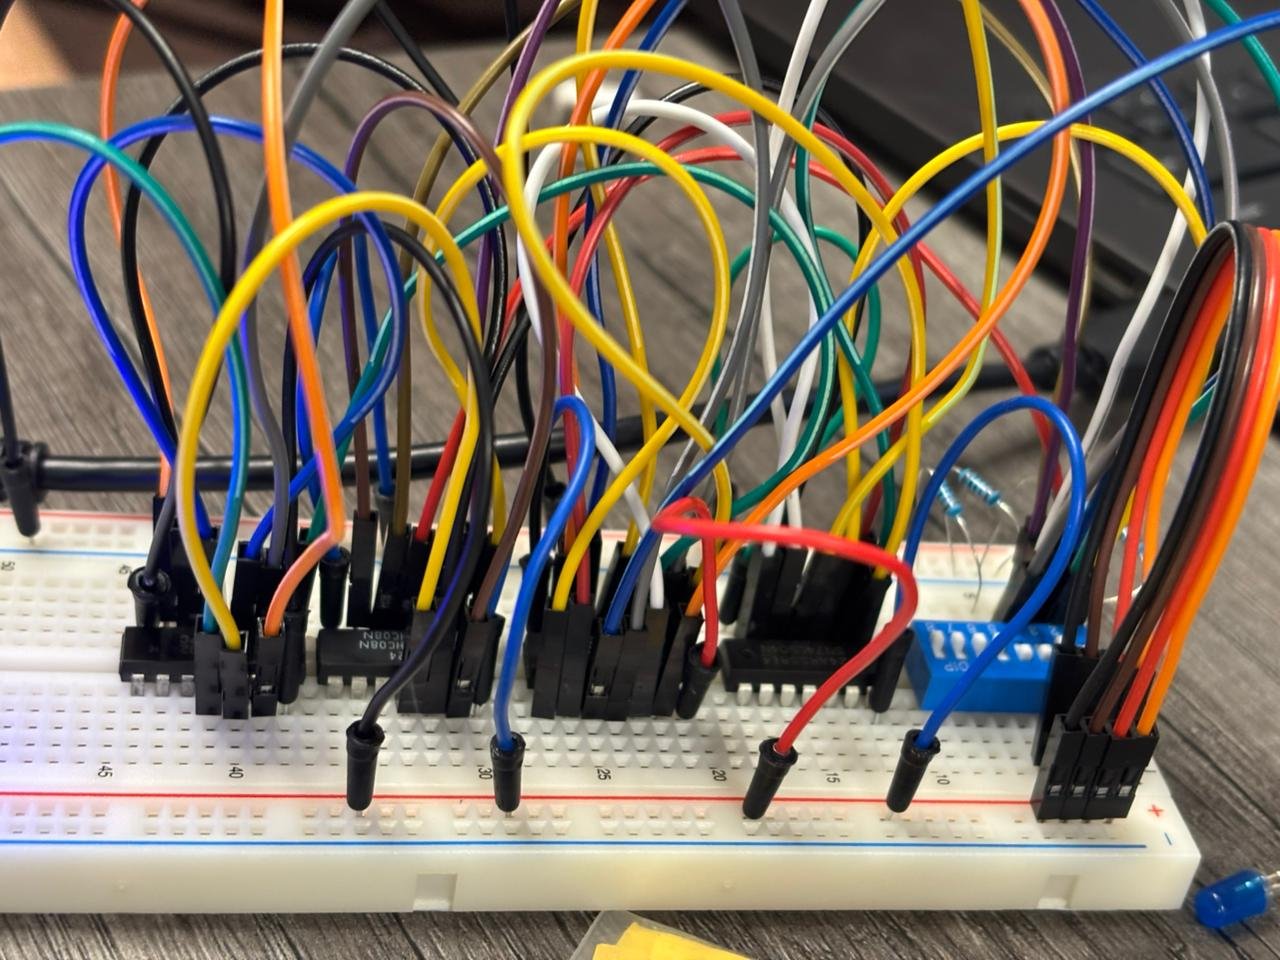
\includegraphics[width=0.4\textwidth]{Point5.jpg}
  \caption{Circuit built in breadboard simulating the Point 5 function.}
  \label{fig:circuit_point_5}
\end{figure}
\subsection{Digital lab experimentation}
After the development of the physical lab, the team developed in Multisim the same circuits developed in the physical lab, to properly organize and correct if necessary any errors.
In the first place, each logic gate was developed and tested:
\begin{figure}[H]
  \centering
  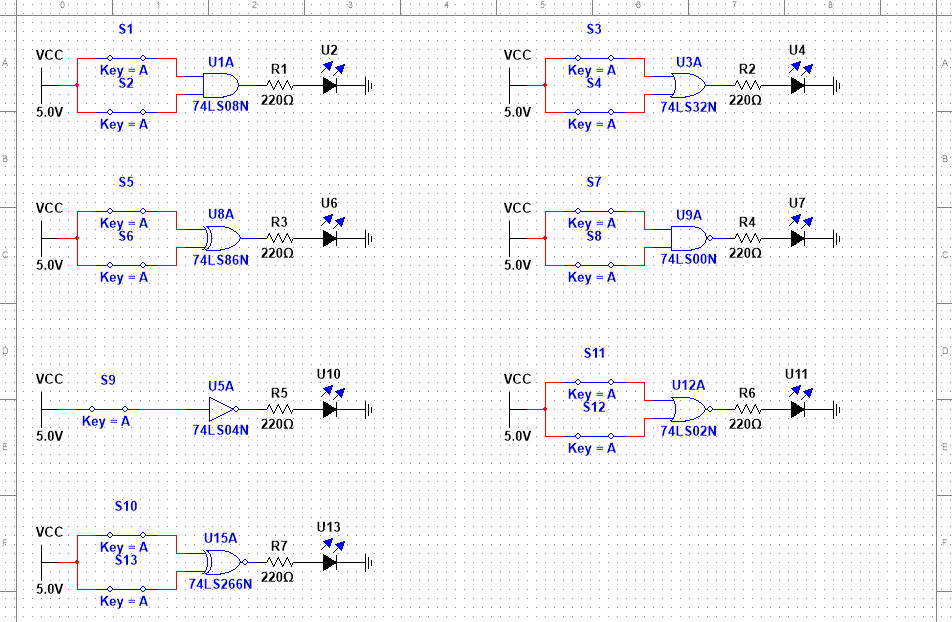
\includegraphics[width=0.4\textwidth]{LogiGates.png}
  \caption{Simulation of the Logic Gates}
  \label{fig:sim_logic_gates}
\end{figure}
And then, the point 5 circuit was designed in the plataform:
\begin{figure}[H]
  \centering
  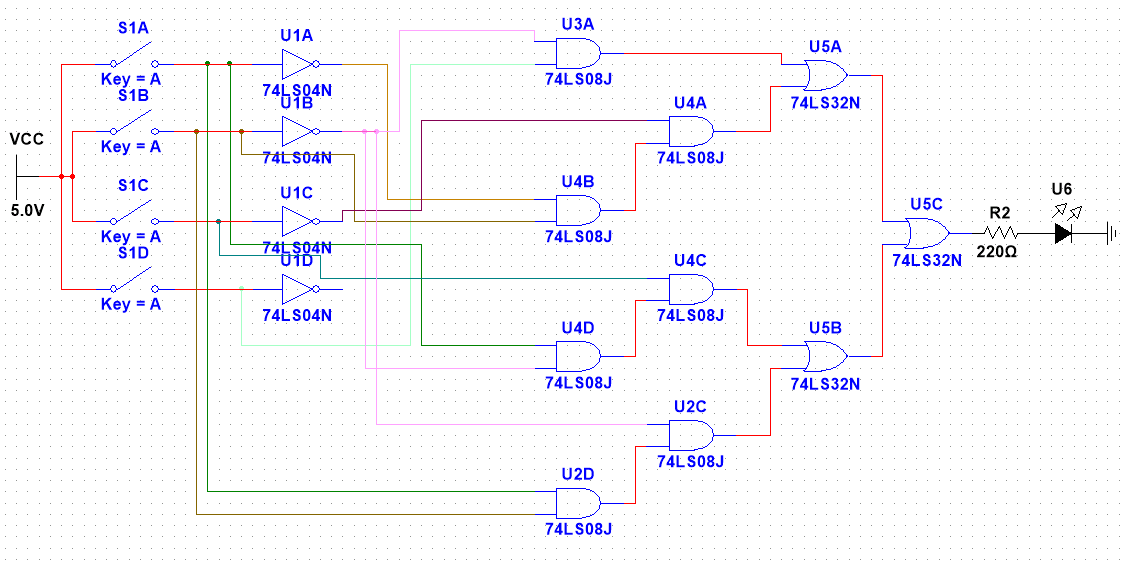
\includegraphics[width=0.4\textwidth]{Point5Multisim.png}
  \caption{Simulation of the point 5 funciton circuit}
  \label{fig:sim_point_5}
\end{figure}

\subsection{Codes}
Finally, the team developed codes in VHDL to prove the functionality of the circuits and function.
The first codes where developed in multiple files, one per logic gate:
\lstinputlisting[language=VHDL,caption=Code 1: AND gate]{codigos/AND.vhd}
\lstinputlisting[language=VHDL,caption=Code 2: OR gate]{codigos/OR.vhd}
\lstinputlisting[language=VHDL,caption=Code 3: NOT gate]{codigos/NOT.vhd}
\lstinputlisting[language=VHDL,caption=Code 4: NAND gate]{codigos/NAND.vhd}
\lstinputlisting[language=VHDL,caption=Code 5: NOR gate]{codigos/NOR.vhd}
\lstinputlisting[language=VHDL,caption=Code 6: XOR gate]{codigos/XOR.vhd}
\lstinputlisting[language=VHDL,caption=Code 7: XNOR gate]{codigos/XNOR.vhd}
After the development of these codes in EDA PLygrounds, the team created a code that showcases the boolean function of point 5:
\lstinputlisting[language=VHDL,caption=Code 8: Point 5 Code]{codigos/point5.vhd}
And to test this code, the team created the following:
\lstinputlisting[language=VHDL,caption=Code 1: Point 5 Testbench]{codigos/point5testbench.vhd}




\section{Analysis} %Análisis de los resultados obtenidos
In the first part, corresponding to the digital inputs (Figure~1), the operation of the circuits with pull-up and pull-down resistors was verified. For the pull-up configuration, when the switch was in the "On" position, the measured voltage was approximately 0~V, corresponding to a low logic state (Low). When the switch was set to "Off", the voltage rose to 4.99~V, identified as a high logic state (High). In the pull-down circuit, the results were the opposite: with the switch activated ("On"), 5.00~V were measured (high state), while with the switch deactivated ("Off"), the voltage dropped to 0~V (low state). These measurements confirm the expected behavior of both methods, showing that the use of pull-up and pull-down resistors ensures a defined logic level at the digital input.

In the second part, corresponding to the digital outputs (Figure~2), the Active Low and Active High circuits were analyzed. For the Active Low configuration, it was observed that the LED remained off when the logic output was at a high level and only turned on when the output was set to a low level. In contrast, in the Active High circuit, the LED turned on with a high logic output and turned off when it was set to a low level. The measured voltages ($\approx$~4.99~V in the active state and 0~V in the inactive state) match the expected values according to the design, confirming the operating principle of both configurations.

Overall, the experimental results are consistent with those obtained in the simulation. The small differences (for example, 4.99~V instead of 5.00~V) are attributed to component tolerances, voltage drops in the connections, and the accuracy of the measuring instruments. Nevertheless, these variations are minimal and do not affect the logical behavior of the circuits. Therefore, it can be concluded that the simulation was a faithful representation of the actual operation, and that the laboratory practice allowed for an experimental validation of the theory.
\clearpage %Asegura que inicie en una nueva página
\section{Conclusions} %Conclusiones del reporte
The lab practice allowed the team to learn the proper usage of both the multimeter abd power supply, ensuring the correct utilization in future circuits.
Additionally, the implementation of both a breadboard circuit and a Multisim simulation, was a showcase of proper understanding of the tools to be used in the class.
Finally, the verification of the correct operation of digital circuits using the multimeter was a success, as the results obtained were consistent with the expected values, confirming the theoretical concepts learned in class.
%%%%%%% Bibliografía %%%%%%%%
\clearpage %Asegura que la bibliografía inicie en una nueva página
\bibliographystyle{bst/IEEEtran} %Estilo de bibliografía NO MODIFICAR PARA MANTENER FORMATO
\bibliography{bib/bibliografia} %Fuentes bibliográficas Se recomienda utilizar un gestor de referencias (zotero, jabref, etc..)
%%%%%%% Bibliografía %%%%%%%%      
\end{document} %Termina el documento
%% Known issues and TODO list%%%
% Warning overfull \hbox en los códigos
% Código en texto blanco y negro y comentarios en negritas => Cambiar a formato en colores